\chapter{GPU Implementierung}
\section{Einleitung}
-implementierung  im rahmen übernommen  ergänzt durch optimierungen in abschnitt () und
-die in abschnitt () vorgstellten immersed boundary methoden
- da auf gpu implementiert mit cuda betrachten wir zunächst hardware architektur


\section{GPU Architektur}

\begin{figure}[!tpb]
  \centering
  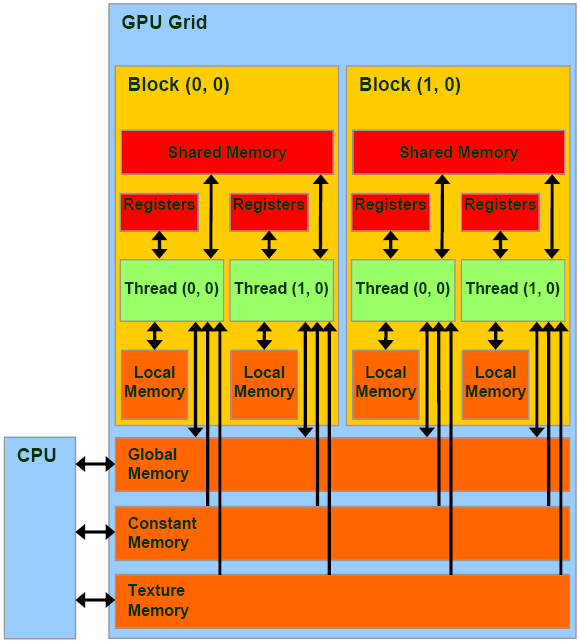
\includegraphics[width=0.6\textwidth]{gfx/cuda/cuda.png}\label{fig:gpu_arch}
  \caption{Speicherlayout einer Nvidia-GPU}
\end{figure}

-bild
-speicher bereiche
-grid layout function call
-threadidx etc

\section{Algorithmus}
-oder so ?
-erläuterung  implementierung
-speicherverwaltung

\section{Optimierung}
- coalesceded
- bank conflicts?
- teilvolumen nicht rechnen

\section{Validierung}
- beispiel rayleigh benard system
- masa
- vgl o2 vs o4 masa cube
- bifurcation


\newpage

